%!TEX root = ../var.tex
\begin{theorem}
\label{th:13.1}
	Функцией единичного скачка или короче функцией
Хевисайда\footnote{Оливер Хевисайд (англ. Oliver Heaviside; 18 мая 1850 — 3 февраля 1925) — английский учёный-
самоучка, инженер, математик и физик. Впервые применил комплексные числа для изучения электрических цепей. Переписал уравнения Максвелла из их первоначальной формы, состоявшей из 20 уравнений
с 12 переменными, к современной форме, состоящей из 4 дифференциальных уравнений, выраженной в
терминах современного векторного анализа. Предложил операционное исчисление (он ввёл обозначение D
для дифференциального оператора) и метод решения дифференциальных уравнений с помощью сведения
к обыкновенным алгебраическим уравнениям. Ввёл термины: «проводимость», «проницаемость», «индуктивность», «импеданс».} называется функция $U : \mathbb{R}\rightarrow \mathbb{R}$, заданная по формуле (см. рис. \ref{fig16})

\begin{equation*}
U(x) = 
 \begin{cases}
   0,x<0\\
   1,x\geqslant 0 
 \end{cases}
\end{equation*}
\end{theorem}

\begin{figure}[H]
	\centering
	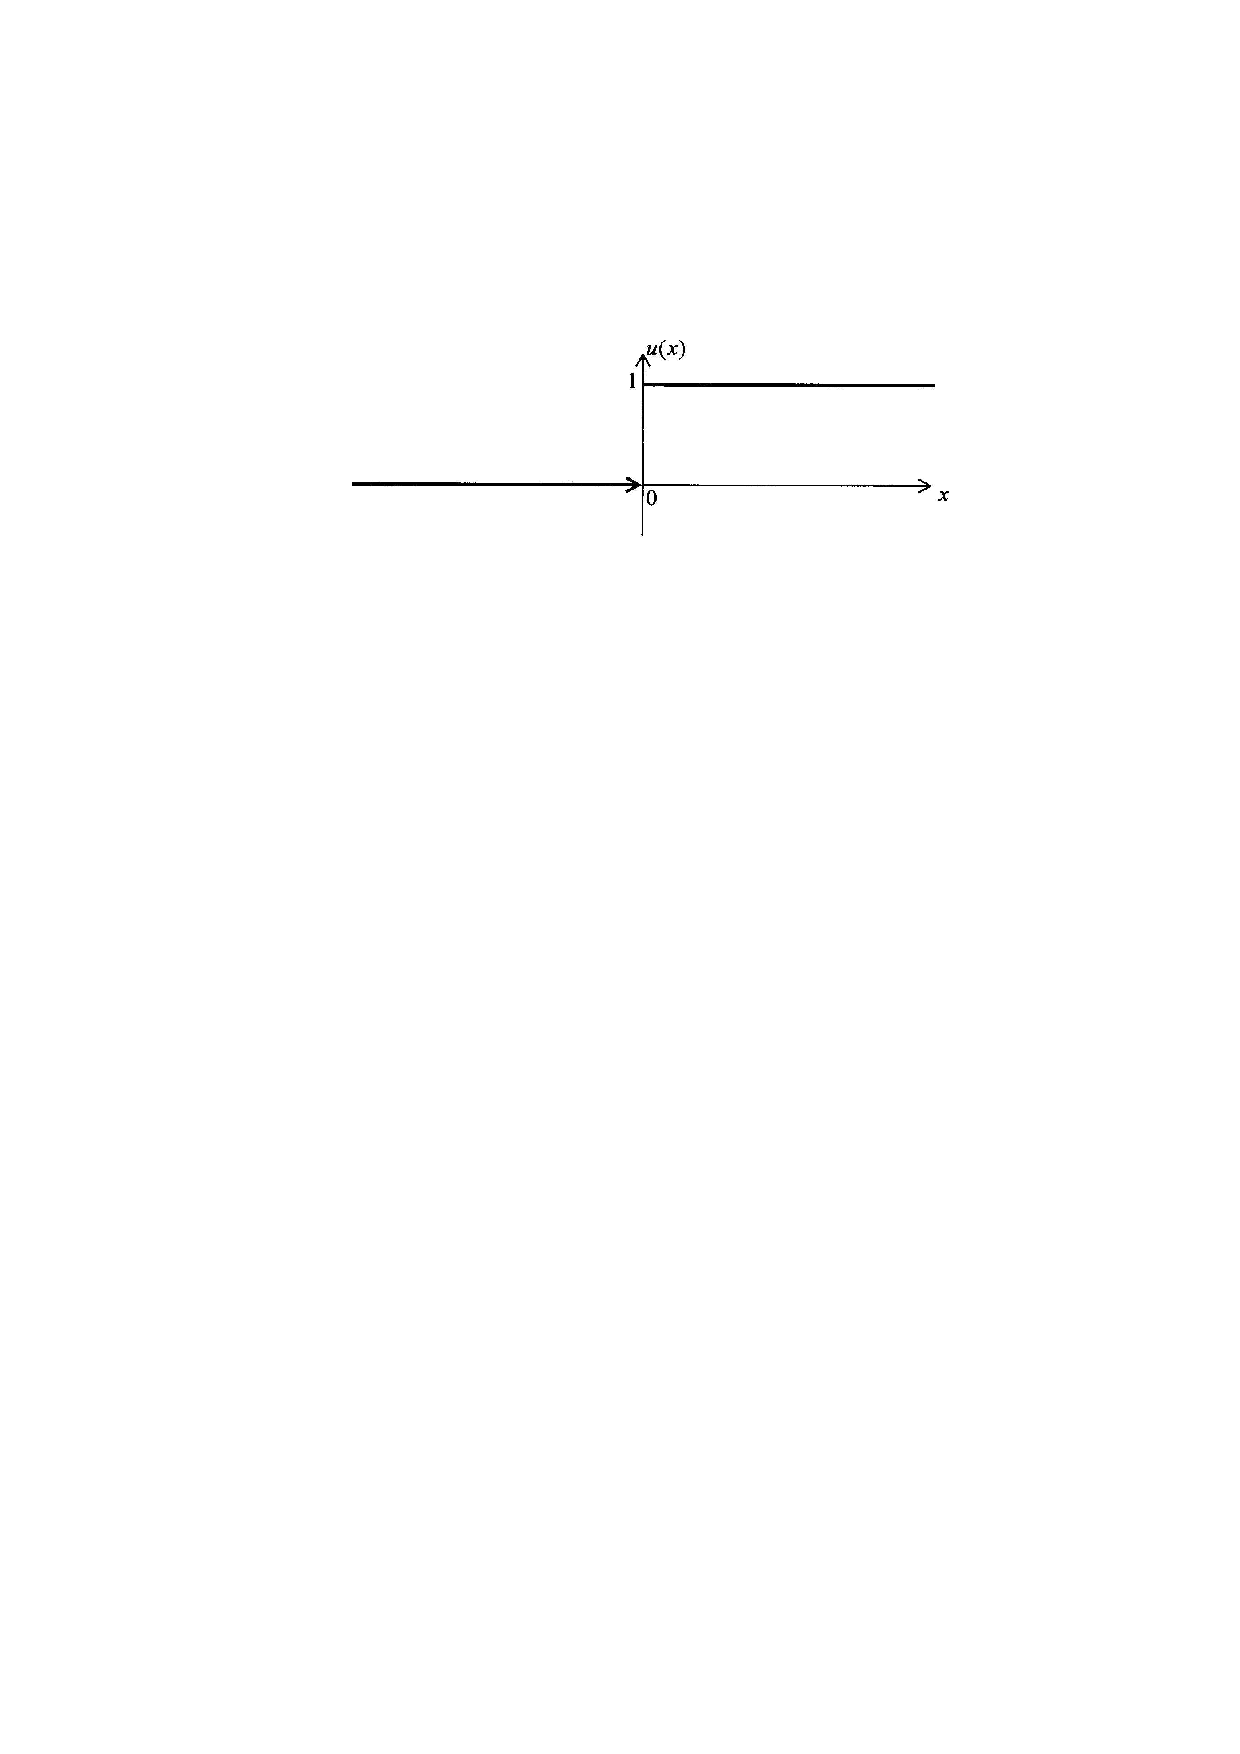
\includegraphics[]{pic/pic16}
	\caption{Функция Хевисайда}
	\label{fig16}
\end{figure}

\begin{example}
\label{ex:13.2}

	Функция Хевисайда полезна для записи в строчку формул (многоэтажных) кусочно заданных функций.

1) Функция единичного импульса единичной длины см. рис. \ref{fig17}.
\begin{equation*}
U(x) = 
 \begin{cases}
   0,x<0\\
   1,x\geqslant 0 
 \end{cases}
 =u(x)-u(x-1).
\end{equation*}

\begin{figure}[H]
	\centering
	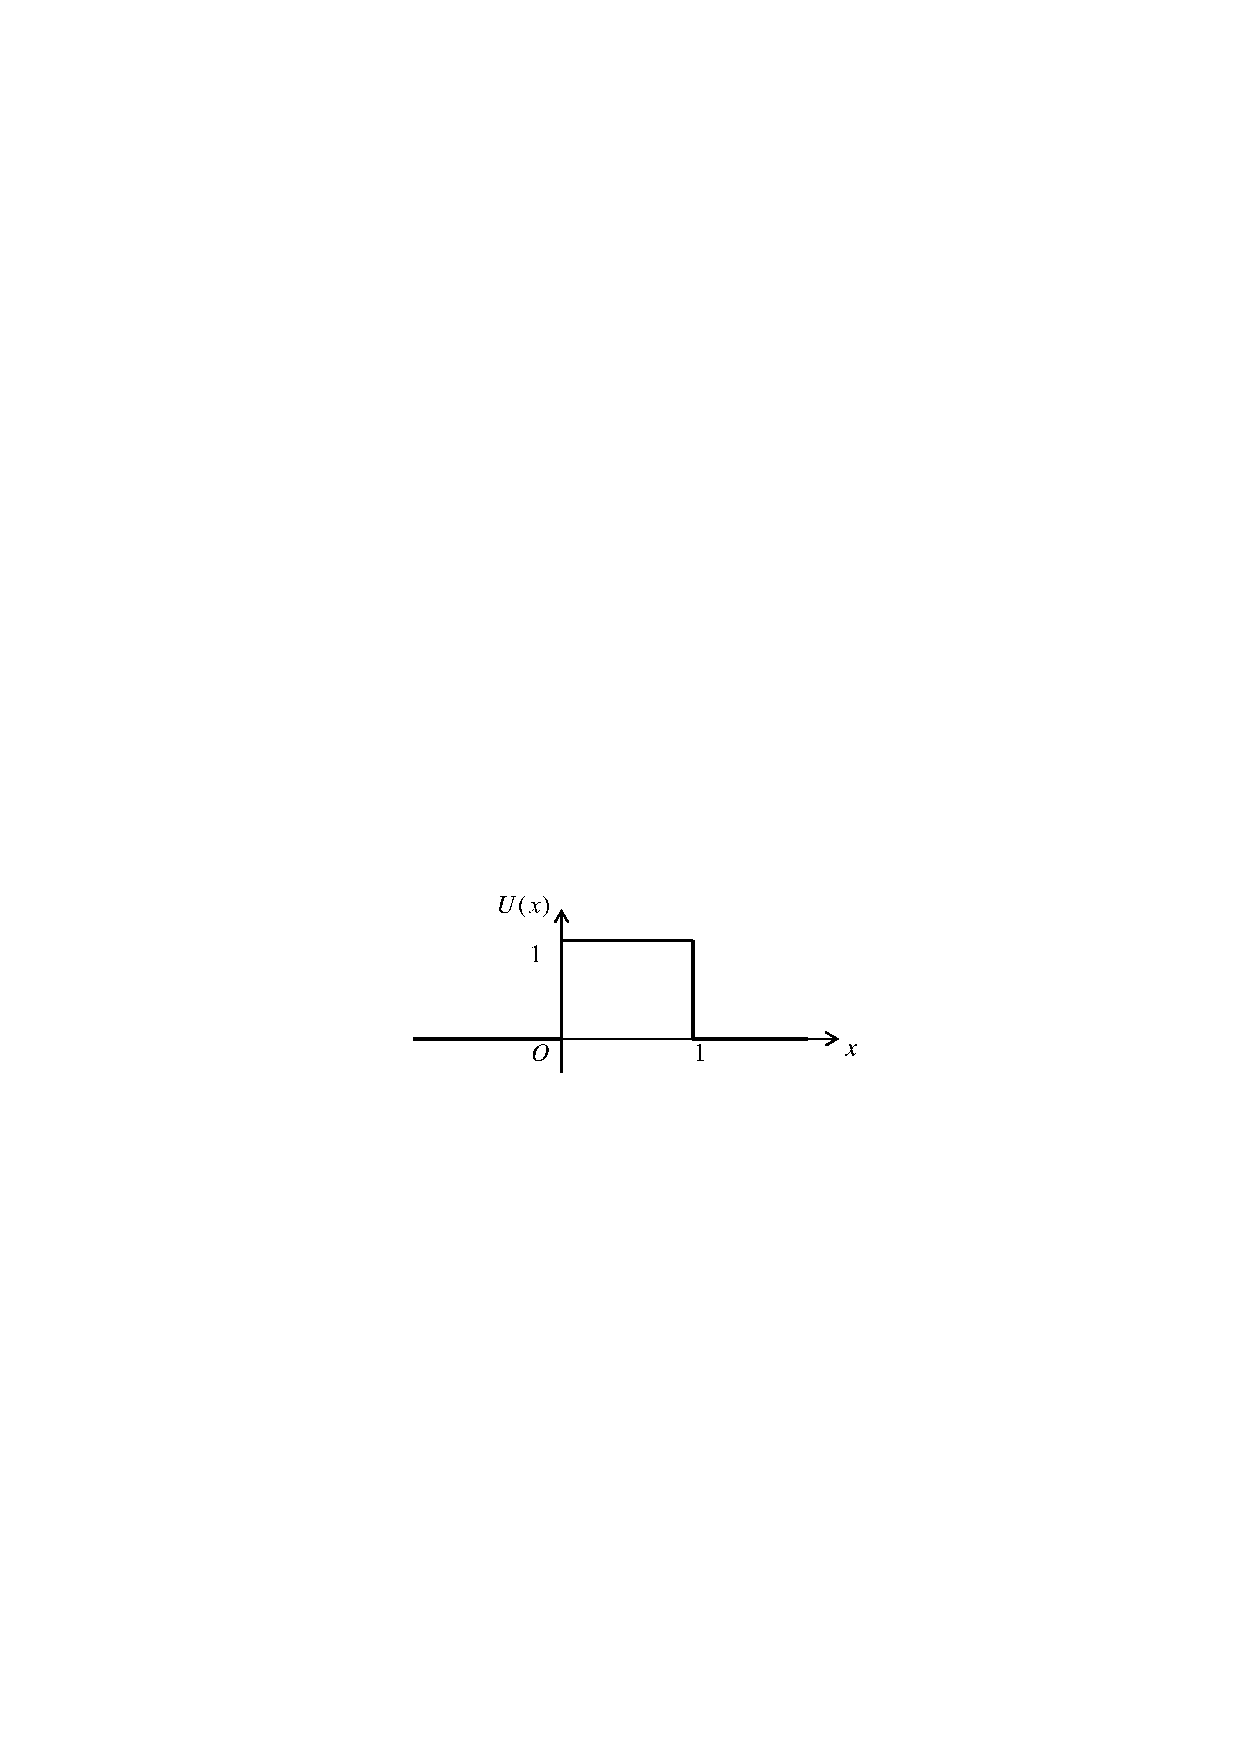
\includegraphics[]{pic/pic17}
	\caption{$U(x) = u(x)-u(x-1)$}
	\label{fig17}
\end{figure}

2) Функция распределения Бернулли, см. рис. \ref{fig10}.
\begin{equation*}
F_{\xi}(x) = 
 \begin{cases}
   0,x<c\\
   1-p,0\leqslant x<1
   p,1\leqslant x
 \end{cases}
 =(1-p)u(x)-pu(x-1).
\end{equation*}

3) Функция равномерного распределения, см. рис. \ref{fig13}
\begin{equation*}
F_{\xi}(x) = 
 \begin{cases}
   0,x<a\\
   \frac{x-a}{b-a},a\leqslant x<b
   1,x\geqslant b
 \end{cases}
 =
 \frac{x-a}{b-a}u(x-a)-\frac{x-a}{b-a}u(x-b)+u(x-b).
\end{equation*}

4)Интеграл от функции Хевисайда.
\begin{equation*}
	\int\limits_{-\infty}^x f(t)u(t)dt=\int\limits_0^xf(t)dt
\end{equation*}
в частности,
\begin{equation*}
	\int\limits_{-\infty}^x u(t)dt=xu(x).
\end{equation*}

\end{example}

\begin{lemma}
\label{lemma:13.3}
	Кусочная функция
\begin{equation*}
	g(x)=
	\begin{cases}
		g_0(x),x<x_0 \\
		g_1(x), x_0\leqslant x<x_1
		\ldots,\ldots
		g_n(x),x_{n-1}\leqslant x<x_n
		g_{n+1}(x), x_n\leqslant x
 	\end{cases}
\end{equation*}
	представима в виде

\begin{gather*}
g(x)=g_0(x)u(x_0-x)+g_1(x)[u(x-x_0)-u(x-x_1)]+\ldots \\
\ldots+g_n(x)[u(x-x_{n-1})-u(x-x_n)]+g_{n+1}(x)u(x-x_n).
\end{gather*}
\end{lemma}

\begin{proof}
	Функция $g(x)$ является суммой следующих функций
	\begin{equation*}
		\widetilde{g}_0(x)=
		\begin{cases}
			g_0(x), x<x_0
			0,x_0\leqslant x
		\end{cases}
		=g_0(x)u(x_0-x),
	\end{equation*}

	\begin{equation*}
		\widetilde{g}_1(x)=
		\begin{cases}
			0(x), x<x_0 \text{ или } x_1\leqslant x \\
			g_1(x),x_0\leqslant x<x_1
		\end{cases}
		=g_1(x)u(x-x_0)-g_1(x)u(x-x_1),
	\end{equation*}

	$\ldots,\ldots$

	\begin{equation*}
		\widetilde{g}_n(x)=
		\begin{cases}
			0(x), x<x_{n-1} \text{ или } x_n\leqslant x \\
			g_n(x),x_{n-1}\leqslant x<x_n
		\end{cases}
		=g_n(x)u(x-x_{n-1})-g_n(x)u(x-x_{n-n}),
	\end{equation*}

		\begin{equation*}
		\widetilde{g}_{n+1}(x)=
		\begin{cases}
			0(x), x<x_{n}\\
			g_n(x),x_{n}\leqslant x<x_n
		\end{cases}
		=g_0(x)u(x-x_{n}).
	\end{equation*}

\end{proof}

\begin{definition}
\label{def:13.4}
	$\delta$-функцией или функцией Дирака называется обобщённая функция
	$\delta : \mathbb{R}\rightarrow\mathbb{R}\cup\{\infty\}$, заданная по формуле

	\begin{equation*}
		\delta(x)=
		\begin{cases}
			0, x \neq 0 \\
			\infty, x=0			
		\end{cases}
	\end{equation*}
	и для любого $\varepsilon > 0$ подчинённая условию $\int\limits^\varepsilon_{-\varepsilon}\delta(x)dx=1$. См. рис. \ref{fig18}.
\end{definition}

\begin{figure}[H]
	\centering
	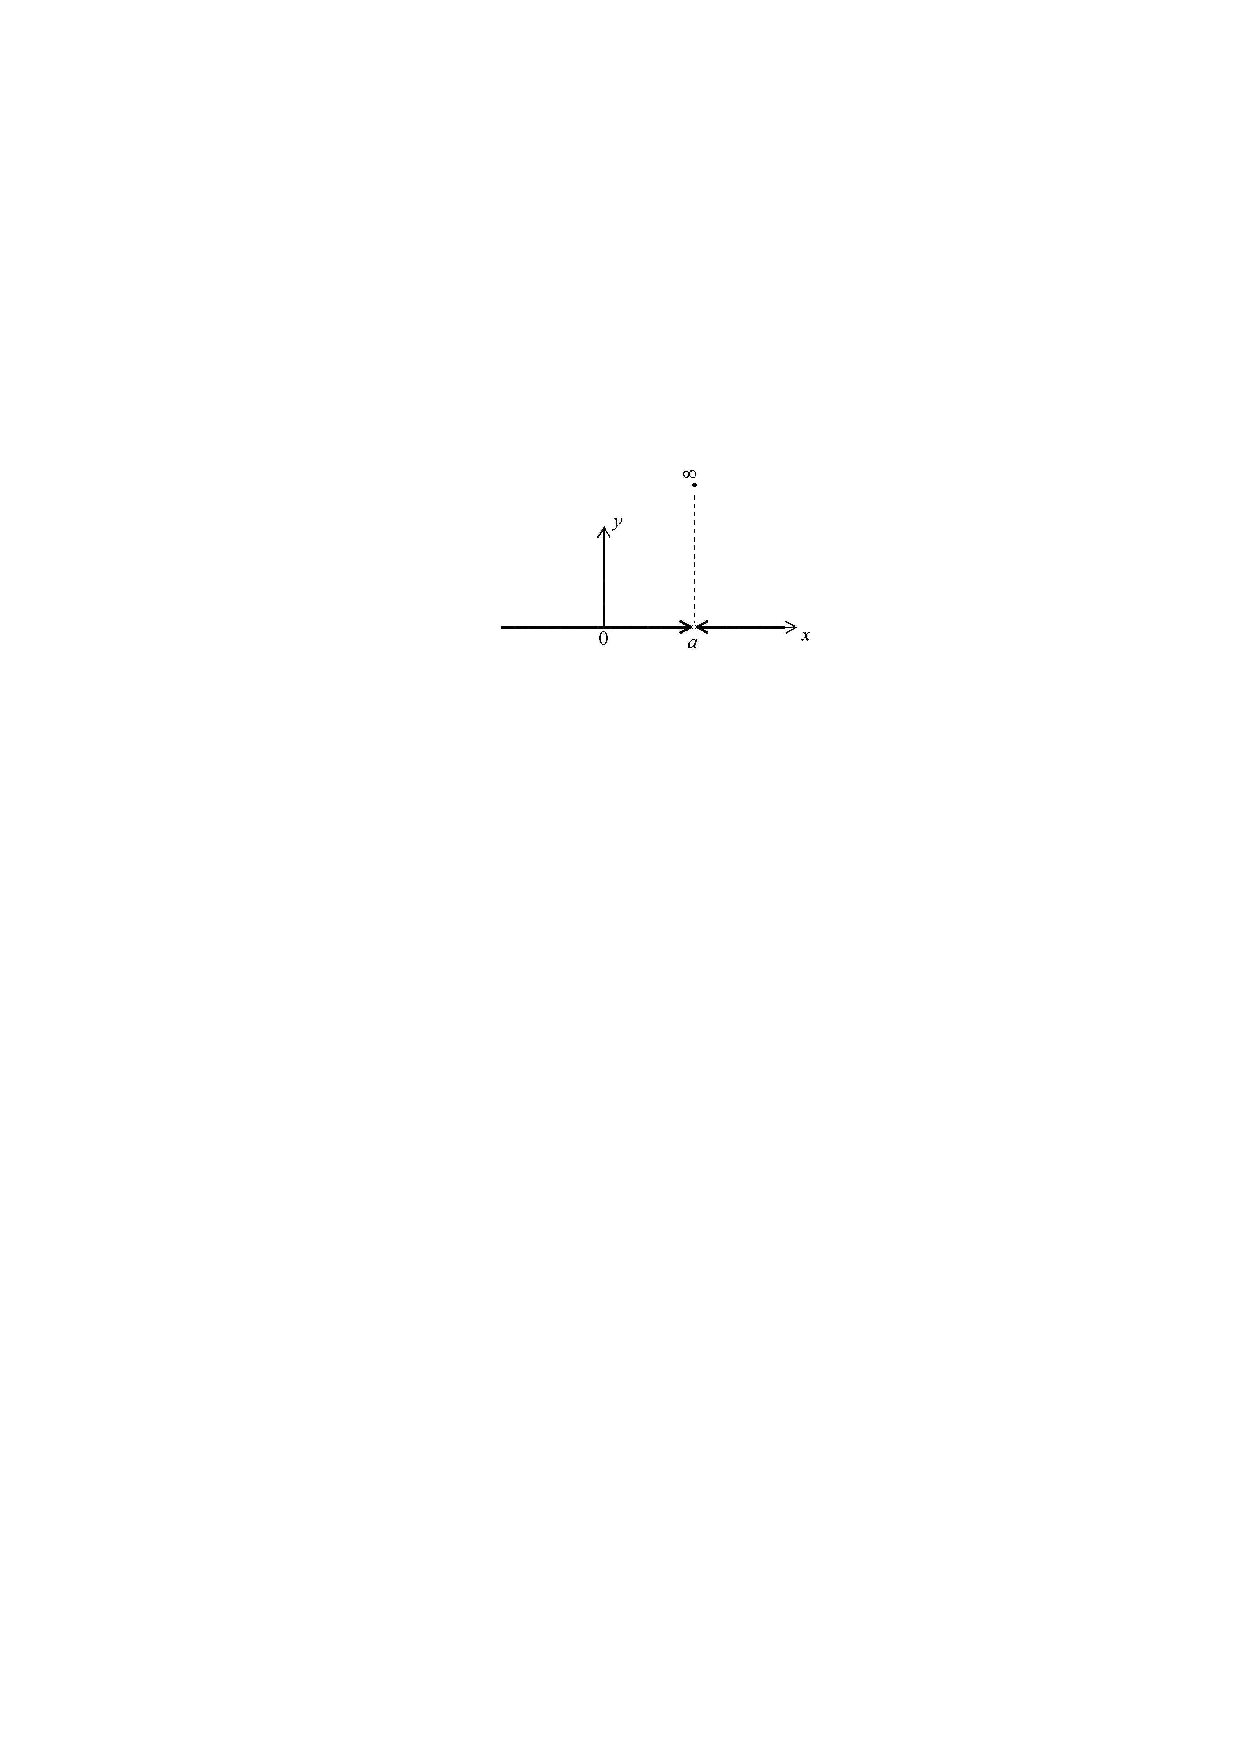
\includegraphics[]{pic/pic18}
	\caption{Функция $y=\delta(x-a)$}
	\label{fig18}
\end{figure}

\begin{prop}
\label{prop:13.5}
\begin{enumerate}
	\item  Для любого $c \in \mathbb{R}$ и любого $\varepsilon > 0$, имеет место формула
\begin{equation*}
	\int\limits_{c-\varepsilon}^{c+\varepsilon}\delta(x-c)dx=1
\end{equation*}
	\item Имеет место формула \begin{equation*}
		u(x)=\int\limits_{-\infty}^x\delta(t)dt
	\end{equation*}
	\item Имеет место формула \begin{equation*}
		u'(x)=\delta(x)
	\end{equation*}
	\item Для любой непрерывной функции $f(x)$ любого $a \in \mathbb{R}$ имеет место тождество
	\begin{equation*}
		f(x)\delta(x-a)=f(a)\delta(x-a).
	\end{equation*}
	\item Для любой непрерывной функции $f(x)$ любого $a \in \mathbb{R}$ имеет место тождество
	\begin{equation*}
		\int\limits_{-\infty}^xf(t)\delta(t-a)dt=f(a)u(x-a),
	\end{equation*}
	в частности
	\begin{equation*}
		\int\limits_{-\infty}^x\delta(t-a)dt=u(x-a)
	\end{equation*}
	\item Если функция $f(x)$ непрерывна и все её нули (корни) $x_1, x_2,\dots , x_k, \dots$ простые (т.е. имеют кратность 1), то
	\begin{equation*}
		\delta(f(x))=\sum\limits_k\frac{\delta(x-x_k)}{|f'(x_k)|}.
	\end{equation*}
	\item Дельта-функция получается при вычислении преобразования Фурье
	от константы:
	\begin{equation*}
		\int\limits_{-\infty}^{\infty}e^{ixt}dt=2\pi \delta(x)
	\end{equation*}
\end{enumerate}
\end{prop}

\begin{example}
\label{ex:13.6}
	1. См.пример 13.2.3. 

	Дано
	\begin{equation*}
		F_{\xi}(x)=\frac{x-a}{b-a}[u(x-a)-u(x-b)]+u(x-b).
	\end{equation*}

	Найти $f_{\xi}(x)$.

	Решение.

	\begin{gather*}
		f_{\xi}(x)=F'_{\xi}(x)=\\
		\\\left(\frac{x-a}{b-a}\right)[u(x-a)-u(x-b)]+\frac{x-a}{b-a}
		[u(x-a)-u(x-b)]+\delta(x-b)=\\
		=\frac{1}{b-a}[u(x-a)-u(x-b)]+\frac{x-a}{b-a}[\delta(x-a)-\delta(x-b)]+\delta(x-b)=
	\end{gather*}
	\begin{gather*}
		=\frac{1}{b-a}[u(x-a)-u(x-b)]+\frac{x-a}{b-a}\delta(x-a)
		-\frac{x-a}{b-a}\delta(x-b)+\delta(x-b)=\\=
		\frac{1}{b-a}[u(x-a)-u(x-b)]+\frac{a-a}{b-a}\delta(x-a)-\frac{b-a}{b-a}\delta(x-b)+\delta(x-b)=\\=\frac{1}{b-a}[u(x-a)-u(x-b)].
	\end{gather*}

	2. Найти плотность вероятности по данной функции распределения
	(см. рис. \ref{fig19})
	
	Дано.
	\begin{equation*}
		F_{\xi}(x)
		\begin{cases}
			0, x<0 \\
			\frac{1}{24}(5x+8), 0\leqslant x<2 \\
			1, x\geqslant 2
		\end{cases}
		=\frac{1}{24}(5x+8)[u(x)-x(x-2)]+u(x-2).
	\end{equation*}

	Решение.

	\begin{gather*}
		f_{\xi}(x)=F'_{\xi}(x)=\\=
		\frac{5}{24}[u(x)-u(x-2)]+\frac{1}{24}(5x+8)[\delta(x)-\delta(x-2)]+\delta(x-2)=\\=
		\frac{5}{24}[u(x)-u(x-2)]+\frac{1}{3}\delta(x)-\frac{3}{4}\delta(x-2)=\\=
		\frac{1}{3}\delta(x)+\frac{5}{24}[u(x)-u(x-2)]+\frac{1}{4}\delta(x-2).
	\end{gather*}
	См. рис. \ref{fig20}
\end{example}
\begin{figure}[H]
	\centering
	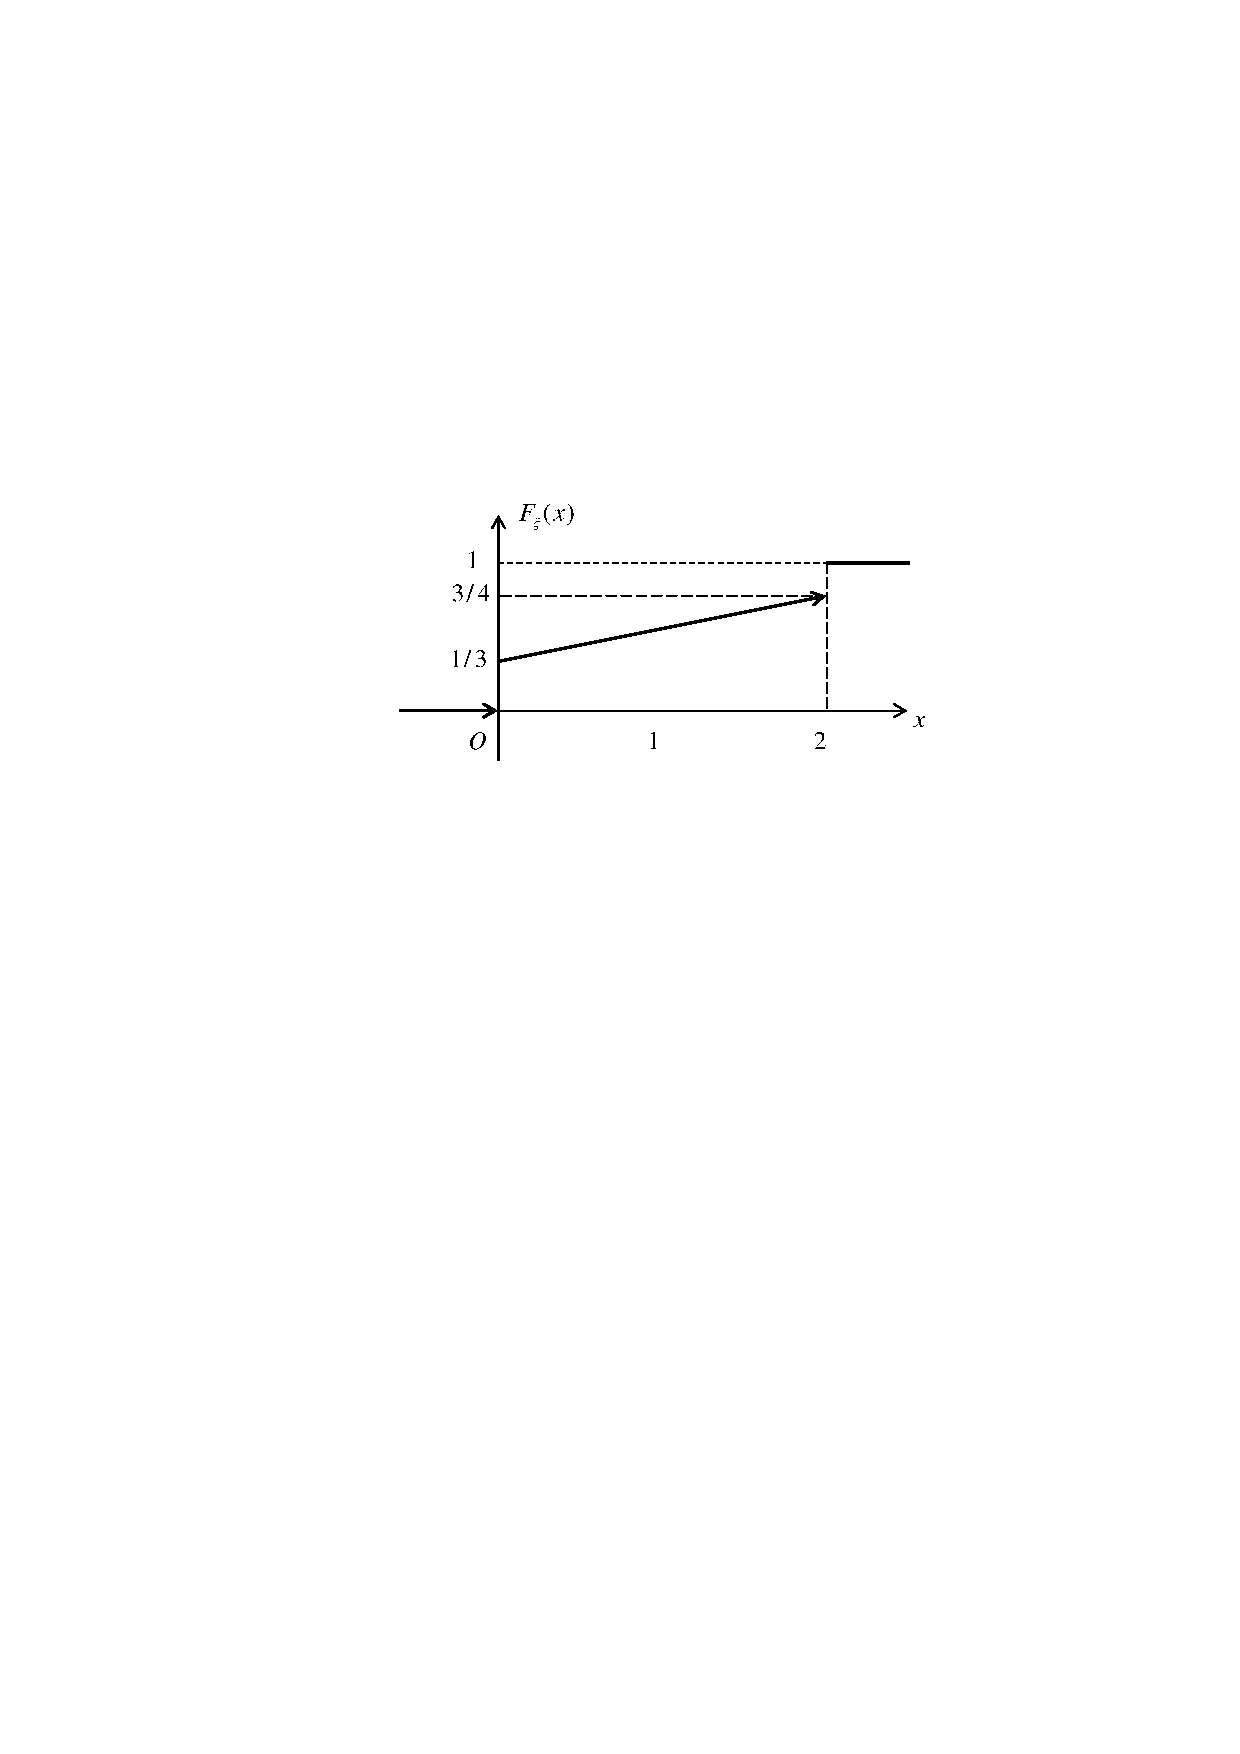
\includegraphics[]{pic/pic19}
	\caption{Функция распределения с двумя скачками}
	\label{fig19}
\end{figure}
\begin{figure}[H]
	\centering
	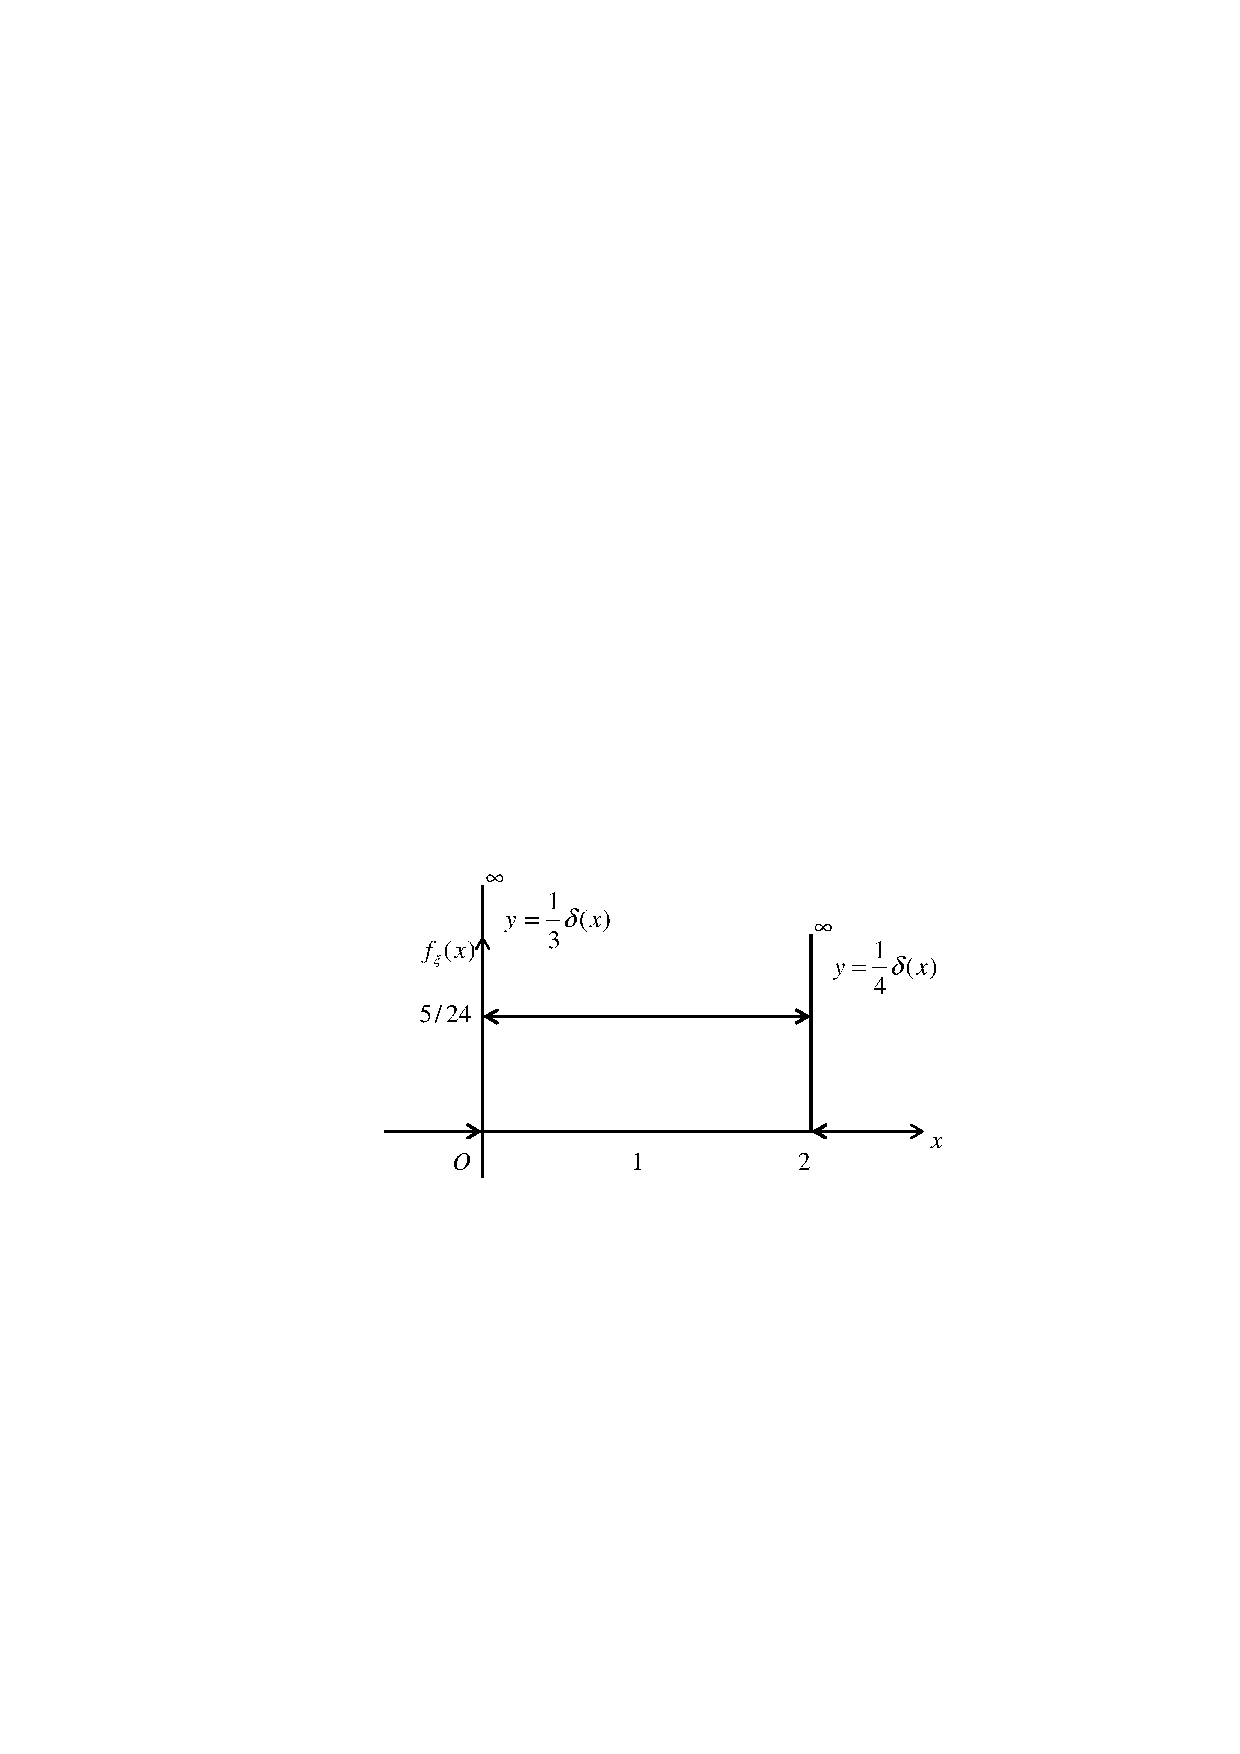
\includegraphics[]{pic/pic20}
	\caption{Площадь под плотностью равна 
				$\frac{1}{3}+\frac{5}{24}\cdot 2+\frac{1}{4}= 1$.}
	\label{fig20}
\end{figure}

\begin{definition}
\label{def:13.6}
	Функции Хевисайда и Дирака и их композиции относятся к классу так называемых обобщённых функций.
\end{definition}